\chapter{Testing Screenshots and Detailed Test Cases}
\label{app:test-cases}

This appendix lists every test case referenced in Chapter~\ref{ch:testing}, together with its identifier. Screenshots of the \ac{E2E} testing are also collected here.

\section{Smart-Contract Test Cases}
\label{apndx:smart-contract-test-cases}
\subsection{Reporting.ts}


\begin{longtable}{p{0.14\textwidth}|p{0.86\textwidth}}
\caption{Reporting contract test cases} \\

  {ID} &   {Purpose} \\
\hline
\endfirsthead
\hline
  {ID} &   {Purpose} \\
\hline
\endhead
T1.1.1 & Authorized relayer submits a report successfully \\
\hline
T1.1.2 & Non-relayer is rejected with \texttt{Unauthorized()} \\
\hline
T1.1.3 & Duplicate nullifier is rejected with \texttt{NullifierAlreadyUsed()} \\
\hline
T1.1.4 & Empty CID is rejected with \texttt{EmptyCID()} \\
\hline
T1.1.5 & Zero report hash is rejected with \texttt{InvalidHash()} \\
\hline
T1.1.6 & Zero nullifier is rejected with \texttt{InvalidNullifier()} \\
\hline
T1.1.7 & Zero pseudonym is rejected with \texttt{InvalidPseudonym()} \\
\hline
T1.1.8 & Report count increments with each submission \\
\hline
T1.1.9 & Phase deadline is set on submission \\
\hline
T1.1.10 & Upvote increments \texttt{validationUpvotes} and emits \texttt{ValidationVoteCast} \\
\hline
T1.1.11 & Downvote increments \texttt{validationDownvotes} \\
\hline
T1.1.12 & Same vote nullifier is rejected with \texttt{NullifierAlreadyUsed()} \\
\hline
T1.1.13 & Same citizen pseudonym cannot vote twice (\texttt{CitizenAlreadyVoted}) \\
\hline
T1.1.14 & Vote after window expiry triggers lazy finalization and is not counted \\
\hline
T1.1.15 & Voting reverts when the report is not in \texttt{PendingValidation} \\
\hline
T1.1.16 & Status moves to \texttt{Open} when upvotes exceed downvotes \\
\hline
T1.1.17 & Status moves to \texttt{CommunityRejected} when downvotes are greater than or equal to upvotes \\
\hline
T1.1.18 & \texttt{finalizeVotingWindow} reverts while the window is still open \\
\hline
T1.1.19 & \texttt{finalizeVotingWindow} succeeds exactly after the window duration elapses \\
\hline
T1.1.20 & \texttt{batchFinalizeVotingWindows} finalizes multiple expired reports together \\
\hline
T1.1.21 & Authority claims an \texttt{Open} report (\texttt{startWork} to \texttt{InProgress}) \\
\hline
T1.1.22 & \texttt{startWork} reverts on the wrong status \\
\hline
T1.1.23 & Authority marks a report solved, moving it to \texttt{PendingVerification} with a phase deadline \\
\hline
T1.1.24 & Wrong authority cannot call \texttt{markAsSolved} (\texttt{Unauthorized}) \\
\hline
T1.1.25 & Authority rejects an issue, moving it to \texttt{PendingRejectionReview} \\
\hline
T1.1.26 & Accept vote increments \texttt{verificationAcceptVotes} \\
\hline
T1.1.27 & Reject vote increments \texttt{verificationRejectVotes} \\
\hline
T1.1.28 & After the window: accept votes greater than or equal to reject votes moves the report to \texttt{Closed} \\
\hline
T1.1.29 & After the window: reject votes greater than accept votes moves the report to \texttt{Reopened} \\
\hline
T1.1.30 & Uphold vote increments \texttt{rejectionUpholdVotes} \\
\hline
T1.1.31 & Appeal vote increments \texttt{rejectionAppealVotes} \\
\hline
T1.1.32 & Uphold votes greater than or equal to appeal votes after the window moves the report to \texttt{Closed} \\
\hline
T1.1.33 & Appeal votes greater than uphold votes after the window moves the report to \texttt{Reopened} \\
\hline
T1.1.34 & \texttt{getAllReports} returns reports newest-first \\
\hline
T1.1.35 & \texttt{getAllReports} with an offset skips the correct number of reports \\
\hline
T1.1.36 & \texttt{getAllReports} with a limit above 100 reverts \texttt{InvalidPagination} \\
\hline
T1.1.37 & \texttt{getReportsByCitizen} returns only reports for the given pseudonym \\
\hline
T1.1.38 & \texttt{getReportCountByCitizen} returns the correct count \\
\hline
T1.1.39 & \texttt{getReportsByIds} returns the correct reports in order \\
\hline
T1.1.40 & \texttt{getReport} with an invalid ID reverts \texttt{InvalidReportId} \\
\hline
T1.1.41 & The authority action log grows correctly across the full lifecycle \\

\end{longtable}

\subsection{EmergencyReporting.ts}

\begin{longtable}{p{0.14\textwidth}|p{0.86\textwidth}}
\caption{Emergency reporting contract test cases} \\

  {ID} &   {Purpose} \\
\hline
\endfirsthead
\hline
  {ID} &   {Purpose} \\
\hline
\endhead
T1.2.1 & Authorized relayer submits; status is immediately \texttt{Open} \\
\hline
T1.2.2 & Nullifier reuse reverts with \texttt{NullifierAlreadyUsed()} \\
\hline
T1.2.3 & Non-relayer is rejected with \texttt{Unauthorized()} \\
\hline
T1.2.4 & Empty CID reverts \texttt{EmptyCID()} \\
\hline
T1.2.5 & Zero report hash reverts \texttt{InvalidHash()} \\
\hline
T1.2.6 & Authority reclassifies the report; \texttt{isReclassified} becomes true and a 30-day penalty is set \\
\hline
T1.2.7 & Penalized citizen cannot submit another emergency (\texttt{EmergencyReportingLocked}) \\
\hline
T1.2.8 & Penalized citizen can submit again after the 30-day penalty expires \\
\hline
T1.2.9 & Reclassifying an already-reclassified report reverts \texttt{InvalidState()} \\
\hline
T1.2.10 & Authority claims an \texttt{Open} emergency, moving it to \texttt{InProgress} \\
\hline
T1.2.11 & Authority resolves an \texttt{InProgress} emergency, moving it to \texttt{Resolved} \\
\hline
T1.2.12 & Authority can resolve directly from \texttt{Open}, bypassing \texttt{InProgress} \\
\hline
T1.2.13 & \texttt{startWork} on a non-\texttt{Open} report reverts \texttt{InvalidState()} \\

\end{longtable}

\subsection{Security.ts}
\label{apndx:security-test-cases}

\begin{longtable}{p{0.14\textwidth}|p{0.86\textwidth}}
\caption{Security and Sybil-resistance test cases} \\

  {ID} &   {Purpose} \\
\hline
\endfirsthead
\hline
  {ID} &   {Purpose} \\
\hline
\endhead
T1.3.1 & All 100 duplicate submission-nullifier replay attempts are rejected \\
\hline
T1.3.2 & A non-relayer account calling \texttt{submitReport} directly is rejected as \texttt{Unauthorized} \\
\hline
T1.3.3 & A second validation vote from the same citizen pseudonym is rejected even with a fresh vote nullifier \\
\hline
T1.3.4 & A second poll vote with the same nullifier is rejected \\
\hline
T1.3.5a & A penalized citizen is blocked from submitting another emergency report for 30 days \\
\hline
T1.3.5b & A penalized citizen can submit again once the 30-day penalty has expired \\
\hline
T1.3.6 & A second verification vote from the same citizen pseudonym is rejected \\

\end{longtable}

\subsection{OpinionPolling.ts}

\begin{longtable}{p{0.14\textwidth}|p{0.86\textwidth}}
\caption{Opinion polling contract test cases} \\

  {ID} &   {Purpose} \\
\hline
\endfirsthead
\hline
  {ID} &   {Purpose} \\
\hline
\endhead
 T1.4.1 & An authorized authority can create a poll \\
\hline
T1.4.2 & Poll creation by a non-authority is reverted \\
\hline
T1.4.3 & Poll creation with a deadline in the past or present is reverted \\
\hline
T1.4.4 & Votes are recorded correctly and \texttt{VoteCast} is emitted \\
\hline
T1.4.5 & Double voting with the same nullifier is reverted \\
\hline
T1.4.6 & Voting after the poll deadline is reverted \\
\hline
T1.4.7 & Voting on a finalized or deactivated poll is reverted \\
\hline
T1.4.8 & Finalizing a poll deactivates it and emits \texttt{PollFinalized} \\
\hline
T1.4.9 & Finalizing a poll that does not exist is reverted \\
\hline
T1.4.10 & Finalizing a poll that is already inactive is reverted \\

\end{longtable}

\subsection{AuthorityMultiSig.ts}

\begin{longtable}{p{0.14\textwidth}|p{0.86\textwidth}}
\caption{Authority multi-signature contract test cases} \\

 {ID} &   {Purpose} \\
\hline
\endfirsthead
\hline
  {ID} &   {Purpose} \\
\hline
\endhead
T1.5.1 & Super Admins can add a new Super Admin through majority vote \\
\hline
T1.5.2 & Super Admins can remove a Super Admin \\
\hline
T1.5.3 & Super Admins can add an authority worker \\
\hline
T1.5.4 & Super Admins can remove an authority worker \\

\end{longtable}

\section{Relayer Test Cases}

\label{apndx:relayer-test-cases}



\begin{longtable}{p{0.14\textwidth}|p{0.86\textwidth}}
\caption{Relayer test cases of ai.oracle.service.spec.ts and app.controller.spec.ts} \\

 {ID} &   {Purpose} \\
\hline
\endfirsthead
\hline
  {ID} &   {Purpose} \\
\hline
\endhead
T2.2.1 & \texttt{canonicalJson()} produces deterministic, sorted output regardless of key order \\
\hline
T2.2.2 & The relayer signature can be recovered and verified by ethers.js \\
\hline
T2.2.3 & A missing \texttt{RELAYER\_PRIVATE\_KEY} logs a warning and fails safely \\
\hline
T2.2.4 & Application bootstrap smoke test (root controller returns a response) \\

\end{longtable}

\begin{longtable}{p{0.14\textwidth}|p{0.86\textwidth}}
\caption{Relayer test cases of reporting.service.spec.ts} \\

 {ID} &   {Purpose} \\
\hline
\endfirsthead
\hline
  {ID} &   {Purpose} \\
\hline
\endhead
T2.3.1 & A valid government signature is accepted and returns a job ID \\
\hline
T2.3.2 & A wrong government signer address is rejected with \texttt{UnauthorizedException} \\
\hline
T2.3.3 & A missing \texttt{zkpSignature} field throws \texttt{BadRequestException} \\
\hline
T2.3.1 & A valid citizen signature is accepted \\
\hline
T2.3.2 & A tampered description causes a signature mismatch, throwing \texttt{UnauthorizedException} \\
\hline
T2.3.3 & A wrong \texttt{citizenPubKey} (address mismatch) causes rejection \\
\hline
T2.3.4 & An image count mismatch throws \texttt{BadRequestException} \\
\hline
T2.3.5 & Malformed \texttt{imageHashes} JSON throws \texttt{BadRequestException} \\
\hline
T2.3.1 & The same address and salt always produce the same pseudonym (deterministic) \\
\hline
T2.3.2 & Different addresses produce different pseudonyms \\
\hline
T2.3.3 & A missing \texttt{PSEUDONYM\_DOMAIN\_SALT} throws \texttt{InternalServerErrorException} \\
\hline
T2.3.1 & A valid vote payload returns a job ID \\
\hline
T2.3.2 & An invalid government ticket for a vote throws \texttt{UnauthorizedException} \\
\hline
T2.3.3 & A tampered vote citizen signature throws \texttt{UnauthorizedException} \\
\hline
T2.3.4 & Missing required vote fields throw \texttt{BadRequestException} \\
\hline
T2.3.1 & A missing \texttt{GOV\_PUBLIC\_ADDRESS} throws on module initialization \\
\end{longtable}


\section{AI Oracle Test Cases}
\label{apndx:ai-test-suite}


\begin{longtable}{p{0.14\textwidth}|p{0.86\textwidth}}
\caption{AI oracle security test cases} \\

 {ID} &   {Purpose} \\
\hline
\endfirsthead
\hline
  {ID} &   {Purpose} \\
\hline
\endhead
T3.1.1 & A fully valid signed request is accepted \\
\hline
T3.1.2 & A missing API key returns 401 or 403 \\
\hline
T3.1.3 & A wrong API key returns 401 or 403 \\
\hline
T3.1.4 & A forged relayer signature returns 401 or 403 \\
\hline
T3.1.5 & A replayed nonce is rejected \\
\hline
T3.1.7 & A file above 5\,MB is rejected \\
\hline
T3.1.8 & A disallowed MIME type (PDF) is rejected \\
\hline
T3.1.9 & More than three files is rejected \\

\end{longtable}

\begin{longtable}{p{0.14\textwidth}|p{0.86\textwidth}}
\caption{AI oracle classification test cases} \\

 {ID} &   {Purpose} \\
\hline
\endfirsthead
\hline
  {ID} &   {Purpose} \\
\hline
\endhead
T3.2.1 & A genuine civic complaint is accepted \\
\hline
T3.2.2 & Hate speech is rejected \\
\hline
T3.2.3 & Commercial spam is rejected \\
\hline
T3.2.4 & Non-civic content is rejected \\
\hline
T3.2.5 & An emergency civic report is accepted \\
\hline
T3.2.6 & A civic report with a valid safe image is accepted \\
\hline
T3.2.7 & A corrupted image attachment is rejected \\
\hline
T3.2.8 & An NSFW image is rejected \\
\hline
T3.2.9 & A civic report with an image containing people is accepted with faces blurred \\
\hline
T3.3.1 & A legitimate governance poll is accepted \\
\hline
T3.3.2 & An inappropriate or non-civic poll is rejected \\
\hline
T3.4.1 & The response always includes a non-empty explanation \\
\hline
T3.4.2 & The response always includes a valid final decision \\
\hline
T3.4.3 & The response structure is consistent across repeated calls \\

\end{longtable}

\section{IPFS Test Cases}
\label{apndx:ipfs-test-suite}

\begin{longtable}{p{0.14\textwidth}|p{0.86\textwidth}}
\caption{IPFS integration test cases} \\

  {ID} &   {Purpose} \\
\hline
\endfirsthead
\hline
  {ID} &   {Purpose} \\
\hline
\endhead
T4.1 & Text-only complaint upload ($\sim$1\,KB) succeeds and returns a CID \\
\hline
T4.2 & Complaint upload with a $\sim$100\,KB image succeeds \\
\hline
T4.3 & Complaint upload with a $\sim$1\,MB image succeeds within a 15-second latency bound \\
\hline
T4.4 & Complaint upload with a $\sim$5\,MB image succeeds \\
\hline
T4.5 & The returned CID is a valid IPFS format \\
\hline
T4.6 & Poll metadata upload to IPFS succeeds \\
\hline
T4.7 & An unreachable IPFS service correctly throws an error \\
\hline
T4.8 & Five concurrent uploads all succeed with no CID collisions \\

\end{longtable}


\section{Blockchain Network Performance Test Cases}
\label{apndx:blockchain-performance-test-cases}
 
\begin{longtable}{p{0.14\textwidth}|p{0.86\textwidth}}
\caption{Blockchain network performance benchmark test cases} \\

  {ID} &   {Purpose} \\
\hline
\endfirsthead
\hline
  {ID} &   {Purpose} \\
\hline
\endhead
T5.1 & Transaction throughput (TPS) is measured by submitting 20 concurrent \texttt{submitReport()} transactions and computing the submission rate \\
\hline
T5.2 & \ac{E2E} submission latency (submit to confirmed) is measured across 5 sequential \texttt{submitReport()} transactions, reporting average, minimum, and maximum \\
\hline
T5.3 & Clique PoA block time is observed by polling the live network for 3 consecutive new blocks and averaging the interval between them \\
\hline
T5.4 & Average gas usage per \texttt{submitReport()} call is measured across 5 submissions \\
\hline
T5.5 & Average gas usage per \texttt{castValidationVote()} call is measured across up to 3 votes on a submitted report \\
\hline
T5.6 & Gas cost of \texttt{batchFinalizeVotingWindows()} is measured for a batch of 10 expired reports, including per-report gas cost \\

\end{longtable}

\section{Manual \ac{E2E} Test Scenarios}
\label{sec:manual-e2e}

The scenarios below covers both citizen workflows and authority workflows through live deployed environment. The citizens can register themselves to the simulated identity simulator via \href{https://drp-gov-sim.internalbuildtools.online/}{https://drp-gov-sim.internalbuildtools.online/} and the dApp can be accessed through \href{https://dapp.internalbuildtools.online/} {https://dapp.internalbuildtools.online/}. Each test scenario records, role, pre-conditions, steps followed, expected results, and the screenshots captured. 


\subsection{Authentication and Access Control}


\subsubsection{Scenario 1 - Citizen Registration }
{Role:} Citizen. \\
{Preconditions:} None

\begin{enumerate}
    
    \item Navigate to \href{https://drp-gov-sim.internalbuildtools.online/}{https://drp-gov-sim.internalbuildtools.online/}, enter a valid identifier and a password, then submit. 
    \item Click on Open Governance DApp.
    \item Observe getting redirected to \href{https://dapp.internalbuildtools.online/} {https://dapp.internalbuildtools.online/}.
\end{enumerate}

\noindent{Expected result:} The citizen is registered successfully and redirected to the dApp. \\
\noindent{Screenshots:} Fig.~\ref{fig:me2e-register}, Fig.~\ref{fig:me2e-register-success}.

\subsubsection{Scenario 2 - Citizen Authentication}
{Role:} Citizen. \\
{Preconditions:} Already registered citizen with a valid government ID and password. 

\begin{enumerate}
    
    \item Open the \ac{DApp} and navigate to login page. 
    \item Select the citizen tab.
    \item Enter a valid GovID and password, then submit. 
    \item Observe redirection to feed page. 
    Open the \ac{DApp} and navigate to \texttt{/login}.
    \item Select the Citizen tab.
    \item Enter a valid GovID and password, then submit.
    \item Confirm that a ticket batch is issued and a citizen seed is returned.
    \item create a PIn and confirm it. 
    \item Observe redirection to \texttt{/feed}.
\end{enumerate}
\noindent{Expected result:} The session is established, citizen only routes are visible and accessible. 

\noindent{Screenshots:} Fig.~\ref{fig:me2e-login}, {fig:me2e-pin-creation}, and  Fig.~\ref{fig:me2e-feed}. 

\subsubsection{Scenario 3 - Invalid Citizen Credentials}
{Role:} Unauthenticated visitor.
{Preconditions:} None.

\begin{enumerate}
    \item Navigate to login screen and select the Citizen tab.
    \item Enter an invalid GovID and/or password, then submit.
\end{enumerate}
\noindent{Expected result:} Authentication fails with a clear error; no ticket batch is issued and no citizen session is created.
\noindent{Screenshots:} Fig.~\ref{fig:m1-3-invalid}.

\paragraph{Scenario M1.4 --- Authority MetaMask connection (happy path).}
\textbf{Role:} Authority worker.
\textbf{Preconditions:} MetaMask is installed, connected to the private PoA network, and the selected account holds \texttt{AUTHORITY\_ROLE}.

\begin{enumerate}
    \item Navigate to \texttt{/login} and select the Authority tab.
    \item Connect MetaMask and approve the connection request.
    \item Open \texttt{/admin} (Authority Portal).
\end{enumerate}
\noindent\textbf{Expected result:} The Authority Dashboard loads with Civic, Emergency, and Polls tabs and report listings.
\noindent\textbf{Screenshots:} Fig.~\ref{fig:m1-4-admin}.

\paragraph{Scenario M1.5 --- Unauthorized access to authority portal (negative path).}
\textbf{Role:} Citizen or unregistered wallet.
\textbf{Preconditions:} A citizen session is active, or MetaMask is connected with a wallet that holds neither authority nor Super Admin roles.

\begin{enumerate}
    \item While authenticated only as a citizen (or with an unregistered wallet), navigate directly to \texttt{/admin}.
\end{enumerate}
\noindent\textbf{Expected result:} RouteGuard denies access and an Access Denied (or equivalent) screen is shown; no authority actions are available.
\noindent\textbf{Screenshots:} Fig.~\ref{fig:m1-5-denied}.

\paragraph{Scenario M1.6 --- Unauthenticated access to citizen routes (negative path).}
\textbf{Role:} Unauthenticated visitor.
\textbf{Preconditions:} No citizen session.

\begin{enumerate}
    \item With no login, navigate to \texttt{/report}.
    \item With no login, navigate to \texttt{/profile}.
\end{enumerate}
\noindent\textbf{Expected result:} Both routes redirect to login or show an access barrier; report submission and profile data are unavailable.
\noindent\textbf{Screenshots:} Fig.~\ref{fig:m1-6-guard}.

\subsection{Standard Report Lifecycle (Happy Path)}

\paragraph{Scenario M2.1 --- Submit standard report through the pipeline.}
\textbf{Role:} Citizen.
\textbf{Preconditions:} Citizen logged in with remaining tickets; emergency toggle off.

\begin{enumerate}
    \item Navigate to \texttt{/report}.
    \item Select a category (for example Road \& Traffic), enter a civic description of at most 1000 characters, attach up to five images, and set a map location.
    \item Submit the report and open \texttt{/notifications}.
    \item Observe ordered progress: AI moderation, then IPFS storage, then blockchain submission, ending in completion.
    \item Open the new report detail page and confirm status \texttt{PendingValidation}.
\end{enumerate}
\noindent\textbf{Expected result:} One ticket is consumed; the report is moderated, stored, and anchored on-chain with status \texttt{PendingValidation}; SSE events complete without failure.
\noindent\textbf{Screenshots:} Fig.~\ref{fig:m2-1-form}, Fig.~\ref{fig:m2-1-notifications}, Fig.~\ref{fig:m2-1-pending}.

\paragraph{Scenario M2.2 --- Community validation to Open.}
\textbf{Role:} Other citizens (validators).
\textbf{Preconditions:} A report from M2.1 is in \texttt{PendingValidation}; voting window has been shortened if needed; at least three other citizens are logged in separately.

\begin{enumerate}
    \item As citizen~B, open the report on \texttt{/issues/[id]} and cast an upvote.
    \item As citizen~C and citizen~D, repeat the upvote.
    \item Wait for the voting window to expire (or trigger finalization), then refresh the report detail.
\end{enumerate}
\noindent\textbf{Expected result:} Status transitions to \texttt{Open}; vote tallies and countdown behaviour match the UI.
\noindent\textbf{Screenshots:} Fig.~\ref{fig:m2-2-vote}, Fig.~\ref{fig:m2-2-open}.

\paragraph{Scenario M2.3 --- Authority claim, update, and mark solved.}
\textbf{Role:} Authority worker.
\textbf{Preconditions:} Report from M2.2 is \texttt{Open}; authority wallet connected.

\begin{enumerate}
    \item Open \texttt{/admin}, locate the report under the Civic tab (Open filter), and open its detail page.
    \item Choose Start Work and confirm; verify status \texttt{InProgress}.
    \item Post an optional progress update.
    \item Choose Mark as Solved and confirm; verify status \texttt{PendingVerification}.
\end{enumerate}
\noindent\textbf{Expected result:} The assigned authority can act; the report moves \texttt{Open} $\rightarrow$ \texttt{InProgress} $\rightarrow$ \texttt{PendingVerification} with an action history entry for each step.
\noindent\textbf{Screenshots:} Fig.~\ref{fig:m2-3-inprogress}, Fig.~\ref{fig:m2-3-pending-verif}.

\paragraph{Scenario M2.4 --- Community verification to Closed.}
\textbf{Role:} Citizens.
\textbf{Preconditions:} Report from M2.3 is \texttt{PendingVerification}; at least two citizens available to vote Accept.

\begin{enumerate}
    \item As two distinct citizens, open the report and cast Accept on the proposed resolution.
    \item Wait for window expiry / finalization and refresh.
\end{enumerate}
\noindent\textbf{Expected result:} Status becomes \texttt{Closed}, completing the canonical standard-report lifecycle described in Chapter~\ref{ch:testing}.
\noindent\textbf{Screenshots:} Fig.~\ref{fig:m2-4-closed}.

\paragraph{Scenario M2.5 --- Citizen profile, my reports, and notifications.}
\textbf{Role:} Reporting citizen from M2.1.
\textbf{Preconditions:} At least one report submitted by this citizen.

\begin{enumerate}
    \item Open \texttt{/profile} and note pseudonym and remaining tickets.
    \item Open \texttt{/my-reports} and confirm the submitted report(s) appear.
    \item Open \texttt{/notifications} and confirm completed (or historical) job statuses are listed.
\end{enumerate}
\noindent\textbf{Expected result:} Profile and my-reports reflect the citizen's pseudonym-scoped data; notifications show pipeline outcomes.
\noindent\textbf{Screenshots:} Fig.~\ref{fig:m2-5-profile}, Fig.~\ref{fig:m2-5-myreports}.

\subsection{Standard Report Alternate and Negative Paths}

\paragraph{Scenario M3.1 --- Community rejection at validation.}
\textbf{Role:} Citizens.
\textbf{Preconditions:} A fresh standard report in \texttt{PendingValidation}.

\begin{enumerate}
    \item Cast enough downvotes so that downvotes are greater than or equal to upvotes by window end.
    \item Finalize / wait for expiry and refresh.
\end{enumerate}
\noindent\textbf{Expected result:} Status becomes \texttt{CommunityRejected}.
\noindent\textbf{Screenshots:} Fig.~\ref{fig:m3-1-rejected}.

\paragraph{Scenario M3.2 --- Authority reject upheld by community.}
\textbf{Role:} Authority, then citizens.
\textbf{Preconditions:} A report in \texttt{Open} or \texttt{InProgress}.

\begin{enumerate}
    \item As authority, choose Reject Issue and confirm; status becomes \texttt{PendingRejectionReview}.
    \item As citizens, cast Uphold votes until upholds are greater than or equal to appeals at window end.
    \item Finalize and refresh.
\end{enumerate}
\noindent\textbf{Expected result:} Status becomes \texttt{Closed} after the rejection is upheld.
\noindent\textbf{Screenshots:} Fig.~\ref{fig:m3-2-review}, Fig.~\ref{fig:m3-2-closed}.

\paragraph{Scenario M3.3 --- Authority reject appealed; report reopened.}
\textbf{Role:} Authority, then citizens.
\textbf{Preconditions:} A report in \texttt{Open} or \texttt{InProgress}.

\begin{enumerate}
    \item As authority, reject the issue to \texttt{PendingRejectionReview}.
    \item As citizens, cast Appeal votes so appeals exceed upholds at window end.
    \item Finalize and refresh; confirm \texttt{Reopened}.
    \item As authority, Start Work again and proceed toward resolution.
\end{enumerate}
\noindent\textbf{Expected result:} Appeal majority returns the report to \texttt{Reopened}; authority can claim it again.
\noindent\textbf{Screenshots:} Fig.~\ref{fig:m3-3-reopened}.

\paragraph{Scenario M3.4 --- Verification reject majority reopens the report.}
\textbf{Role:} Authority, then citizens.
\textbf{Preconditions:} A report in \texttt{PendingVerification} after Mark as Solved.

\begin{enumerate}
    \item As citizens, cast Reject votes so rejects exceed accepts at window end.
    \item Finalize and refresh.
\end{enumerate}
\noindent\textbf{Expected result:} Status becomes \texttt{Reopened}.
\noindent\textbf{Screenshots:} Fig.~\ref{fig:m3-4-verif-reopen}.

\paragraph{Scenario M3.5 --- Client-side submission validation (negative path).}
\textbf{Role:} Citizen.
\textbf{Preconditions:} Citizen logged in at \texttt{/report}.

\begin{enumerate}
    \item Attempt submit with an empty description.
    \item Attempt submit without a map location.
    \item Attempt to attach more than five images.
    \item Attempt a description longer than 1000 characters (if the UI allows typing past the limit, confirm it blocks or truncates).
\end{enumerate}
\noindent\textbf{Expected result:} Each invalid attempt is blocked in the client with a validation message; no relayer job is created.
\noindent\textbf{Screenshots:} Fig.~\ref{fig:m3-5-validation}.

\paragraph{Scenario M3.6 --- AI moderation rejection (negative path).}
\textbf{Role:} Citizen.
\textbf{Preconditions:} Citizen logged in with remaining tickets.

\begin{enumerate}
    \item Submit a report whose text or image is expected to fail moderation (for example hate speech, spam, non-civic content, or an unsafe image sample used in AI testing).
    \item Open \texttt{/notifications} and wait for the AI stage outcome.
\end{enumerate}
\noindent\textbf{Expected result:} The job fails at AI moderation with a rejection status; the report is not anchored on-chain as an accepted civic issue.
\noindent\textbf{Screenshots:} Fig.~\ref{fig:m3-6-ai-reject}.

\paragraph{Scenario M3.7 --- Duplicate geo and category warning.}
\textbf{Role:} Citizen.
\textbf{Preconditions:} An existing open or recent report near a known location and category.

\begin{enumerate}
    \item Start a new report with the same category and a location within about 1\,km of the existing report.
    \item Observe the duplicate-warning modal and any preview of nearby reports.
    \item Either cancel or acknowledge and continue, depending on the intended test outcome.
\end{enumerate}
\noindent\textbf{Expected result:} The duplicate warning appears before final submission; the citizen can review nearby reports.
\noindent\textbf{Screenshots:} Fig.~\ref{fig:m3-7-duplicate}.

\paragraph{Scenario M3.8 --- Double vote and ticket exhaustion (negative path).}
\textbf{Role:} Citizen.
\textbf{Preconditions:} A report in an active voting phase; a citizen who has already voted, and optionally a citizen with tickets nearly exhausted.

\begin{enumerate}
    \item Attempt a second vote on the same report with the same citizen session.
    \item Continue casting ticket-consuming actions until the ticket batch is exhausted, then attempt another action.
\end{enumerate}
\noindent\textbf{Expected result:} The second vote is rejected (nullifier or citizen-already-voted); exhausted tickets require re-login to obtain a new batch before further actions succeed.
\noindent\textbf{Screenshots:} Fig.~\ref{fig:m3-8-double-vote}.

\subsection{Emergency Flows}

\paragraph{Scenario M4.1 --- Emergency report submission (happy path).}
\textbf{Role:} Citizen.
\textbf{Preconditions:} Citizen logged in; citizen is not under an emergency-channel penalty.

\begin{enumerate}
    \item On \texttt{/report}, enable the Urgent/Emergency toggle.
    \item Confirm the emergency consent modal.
    \item Complete category, description, location, and optional images, then submit.
    \item Track notifications through AI, IPFS, and chain stages.
\end{enumerate}
\noindent\textbf{Expected result:} The report is created on the emergency path with status \texttt{Open} immediately (validation skipped).
\noindent\textbf{Screenshots:} Fig.~\ref{fig:m4-1-consent}, Fig.~\ref{fig:m4-1-open}.

\paragraph{Scenario M4.2 --- Authority resolve emergency.}
\textbf{Role:} Authority worker.
\textbf{Preconditions:} An emergency report in \texttt{Open} (from M4.1).

\begin{enumerate}
    \item Open the Authority Dashboard Emergency tab and open the report.
    \item Optionally Start Work (\texttt{InProgress}), then Resolve; or Resolve directly from \texttt{Open}.
\end{enumerate}
\noindent\textbf{Expected result:} Status becomes \texttt{Resolved}.
\noindent\textbf{Screenshots:} Fig.~\ref{fig:m4-2-resolved}.

\paragraph{Scenario M4.3 --- Reclassify false emergency.}
\textbf{Role:} Authority worker.
\textbf{Preconditions:} A separate emergency report that should be treated as non-urgent abuse of the channel.

\begin{enumerate}
    \item On the emergency report detail, choose Downgrade / Reclassify (false emergency) and confirm.
\end{enumerate}
\noindent\textbf{Expected result:} Status becomes \texttt{Reclassified}; the reporting citizen receives a 30-day lock on the emergency channel.
\noindent\textbf{Screenshots:} Fig.~\ref{fig:m4-3-reclassified}.

\paragraph{Scenario M4.4 --- Emergency penalty enforcement (negative path).}
\textbf{Role:} Penalized citizen.
\textbf{Preconditions:} Citizen from M4.3 is within the 30-day emergency lock.

\begin{enumerate}
    \item Attempt to submit another emergency report.
    \item Submit a standard (non-emergency) report with the same account.
\end{enumerate}
\noindent\textbf{Expected result:} The second emergency submission is blocked; the standard report is still accepted through the normal pipeline.
\noindent\textbf{Screenshots:} Fig.~\ref{fig:m4-4-penalty}.

\paragraph{Scenario M4.5 --- Emergency without consent (negative path).}
\textbf{Role:} Citizen.
\textbf{Preconditions:} Citizen on \texttt{/report}.

\begin{enumerate}
    \item Enable the Emergency toggle, then dismiss or cancel the consent modal without confirming.
    \item Attempt to submit without having accepted consent.
\end{enumerate}
\noindent\textbf{Expected result:} Emergency submission does not proceed without consent.
\noindent\textbf{Screenshots:} Fig.~\ref{fig:m4-5-cancel-consent}.

\subsection{Opinion Polling}

\paragraph{Scenario M5.1 --- Authority creates a poll.}
\textbf{Role:} Authority worker.
\textbf{Preconditions:} Authority wallet connected.

\begin{enumerate}
    \item Navigate to \texttt{/polls/create}.
    \item Enter poll metadata (question, options / true--false as applicable) and submit.
    \item Confirm metadata is uploaded and the on-chain poll is created.
    \item Verify the poll appears on \texttt{/polls} or the feed for citizens.
\end{enumerate}
\noindent\textbf{Expected result:} Poll is visible to citizens and listed under the Authority Polls tab.
\noindent\textbf{Screenshots:} Fig.~\ref{fig:m5-1-create}, Fig.~\ref{fig:m5-1-list}.

\paragraph{Scenario M5.2 --- Citizens vote and authority finalizes.}
\textbf{Role:} Citizens, then authority.
\textbf{Preconditions:} Active poll from M5.1 within its deadline.

\begin{enumerate}
    \item As two or more citizens, open the poll and cast a vote.
    \item As authority, finalize the poll from the Admin Polls tab when ready.
\end{enumerate}
\noindent\textbf{Expected result:} Votes are recorded via the relayer; finalized poll no longer accepts new votes and shows a completed state.
\noindent\textbf{Screenshots:} Fig.~\ref{fig:m5-2-vote}, Fig.~\ref{fig:m5-2-finalized}.

\paragraph{Scenario M5.3 --- Poll access and double-vote controls (negative path).}
\textbf{Role:} Citizen.
\textbf{Preconditions:} Active poll; citizen already voted once.

\begin{enumerate}
    \item As a citizen, navigate to \texttt{/polls/create} and confirm access is denied.
    \item Attempt a second vote on the same poll with the same citizen.
\end{enumerate}
\noindent\textbf{Expected result:} Citizens cannot create official polls; double vote is rejected (nullifier reuse).
\noindent\textbf{Screenshots:} Fig.~\ref{fig:m5-3-denied}.

\subsection{Super Admin Governance}

\paragraph{Scenario M6.1 --- Multisig proposal and majority approval (happy path).}
\textbf{Role:} Super Admins.
\textbf{Preconditions:} At least two Super Admin wallets; useful first action is setting a short voting-window duration for later M2/M3 scenarios.

\begin{enumerate}
    \item As Super Admin~A, open \texttt{/super-admin} and submit a proposal (for example set voting-window duration, or add/remove an authority).
    \item Confirm the proposal appears as active and the submitter's vote is recorded.
    \item As Super Admin~B, approve the same proposal until majority quorum $Q=\lfloor N/2\rfloor+1$ is reached.
    \item Confirm execution and verify the on-chain configuration or roster change.
\end{enumerate}
\noindent\textbf{Expected result:} The change applies only after majority approval; the dashboard reflects the new config or roster.
\noindent\textbf{Screenshots:} Fig.~\ref{fig:m6-1-propose}, Fig.~\ref{fig:m6-1-executed}.

\paragraph{Scenario M6.2 --- Unilateral change and unauthorized access (negative path).}
\textbf{Role:} Single Super Admin; then a non--Super Admin.
\textbf{Preconditions:} At least two Super Admins registered so quorum is greater than one.

\begin{enumerate}
    \item As a single Super Admin, submit a proposal and leave it without a second approval; confirm it is not executed.
    \item As a citizen or ordinary authority wallet, navigate to \texttt{/super-admin}.
\end{enumerate}
\noindent\textbf{Expected result:} Unilateral proposals do not execute; non--Super Admin users are denied the Super Admin dashboard.
\noindent\textbf{Screenshots:} Fig.~\ref{fig:m6-2-denied}.

\section{Testing Screenshots}
\label{sec:testing-screenshots}

The figures below correspond to the manual scenarios in Section~\ref{sec:manual-e2e}. Replace each placeholder box with a captured screenshot by placing the image under \texttt{Images/Appendix/} and uncommenting the matching \texttt{\textbackslash includegraphics} line.

\subsection{Authentication Screenshots}

\begin{figure}[H]
    \centering
    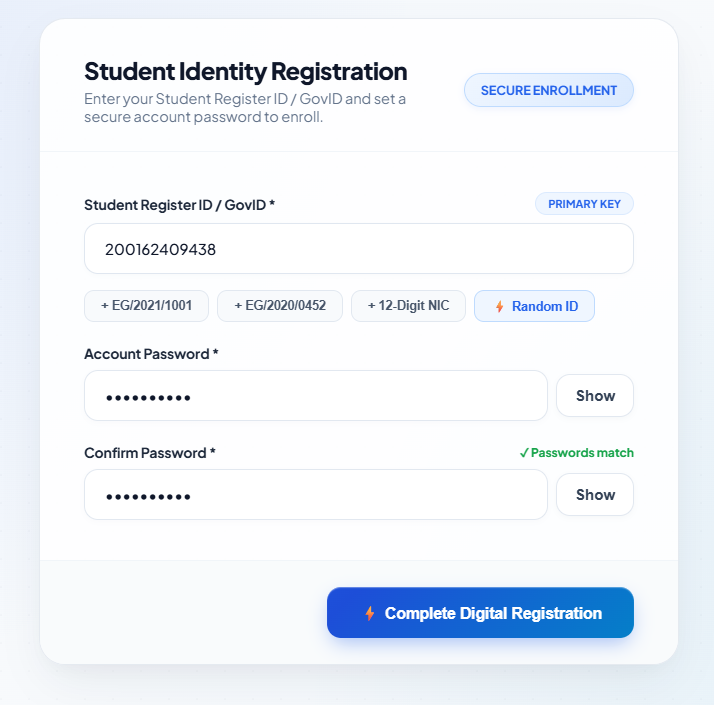
\includegraphics[width=0.85\textwidth]{Images/Appendix/me2e/register.png}
    %\fbox{\parbox{0.85\textwidth}{\centering\vspace{3.5cm}[Screenshot M1.1-a: Citizen login]\vspace{3.5cm}}}
    \caption{Registration screen of government identity simulator}
    \label{fig:me2e-register}
\end{figure}

\begin{figure}[H]
    \centering
    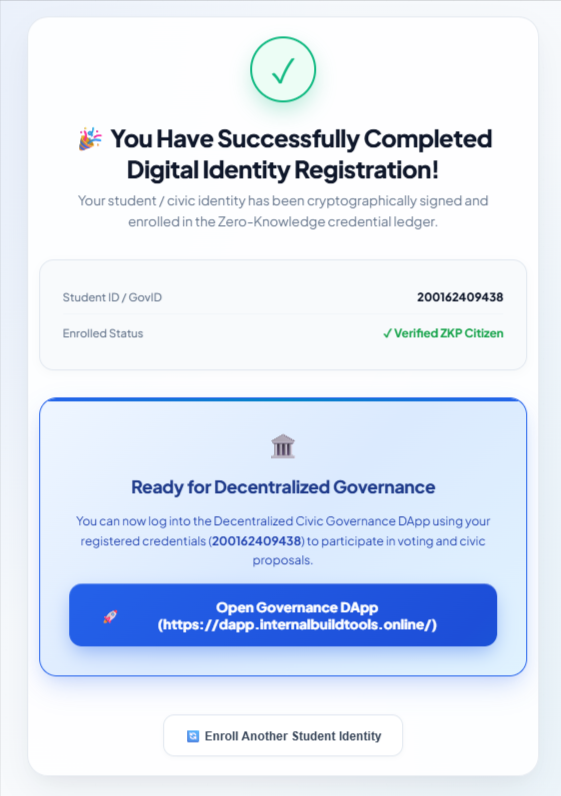
\includegraphics[width=0.85\textwidth]{Images/Appendix/me2e/register-success.png}
   % \fbox{\parbox{0.85\textwidth}{\centering\vspace{3.5cm}[Screenshot M1.1-a: Citizen login]\vspace{3.5cm}}}
    \caption{Successfull registration of a citizen via government identity simulator}
    \label{fig:me2e-register-success}
\end{figure}



\begin{figure}[H]
    \centering
    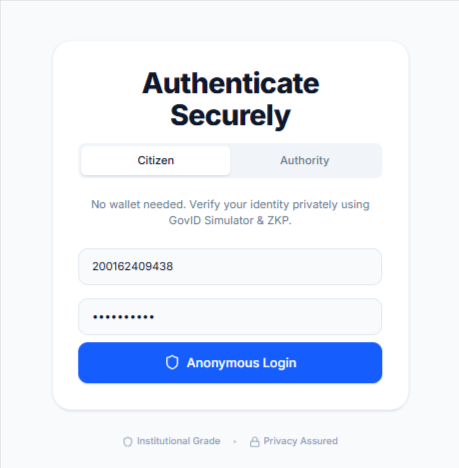
\includegraphics[width=0.85\textwidth]{Images/Appendix/me2e/login-screen.png}
    %\fbox{\parbox{0.85\textwidth}{\centering\vspace{3.5cm}[Screenshot M1.1-a: Citizen login]\vspace{3.5cm}}}
    \caption{Citizen login to the DApp}
    \label{fig:me2e-login}
\end{figure}

\begin{figure}[H]
    \centering
    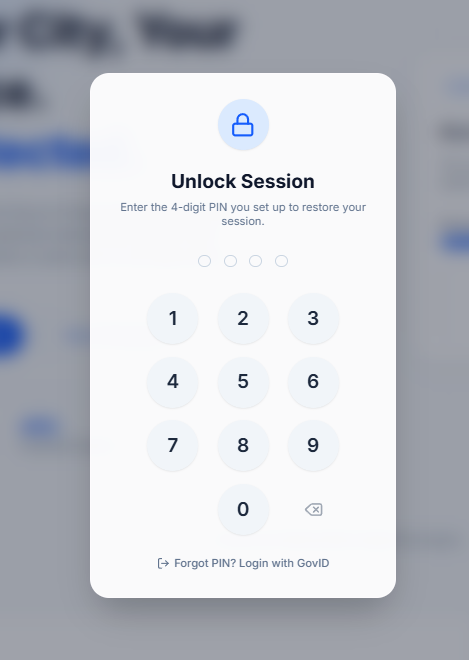
\includegraphics[width=0.85\textwidth]{Images/Appendix/me2e/pin-creation.png}
    %\fbox{\parbox{0.85\textwidth}{\centering\vspace{3.5cm}[Screenshot M1.1-a: Citizen login]\vspace{3.5cm}}}
    \caption{PIN creation screen}
    \label{fig:me2e-pin-creation}
\end{figure}

\begin{figure}[H]
    \centering
    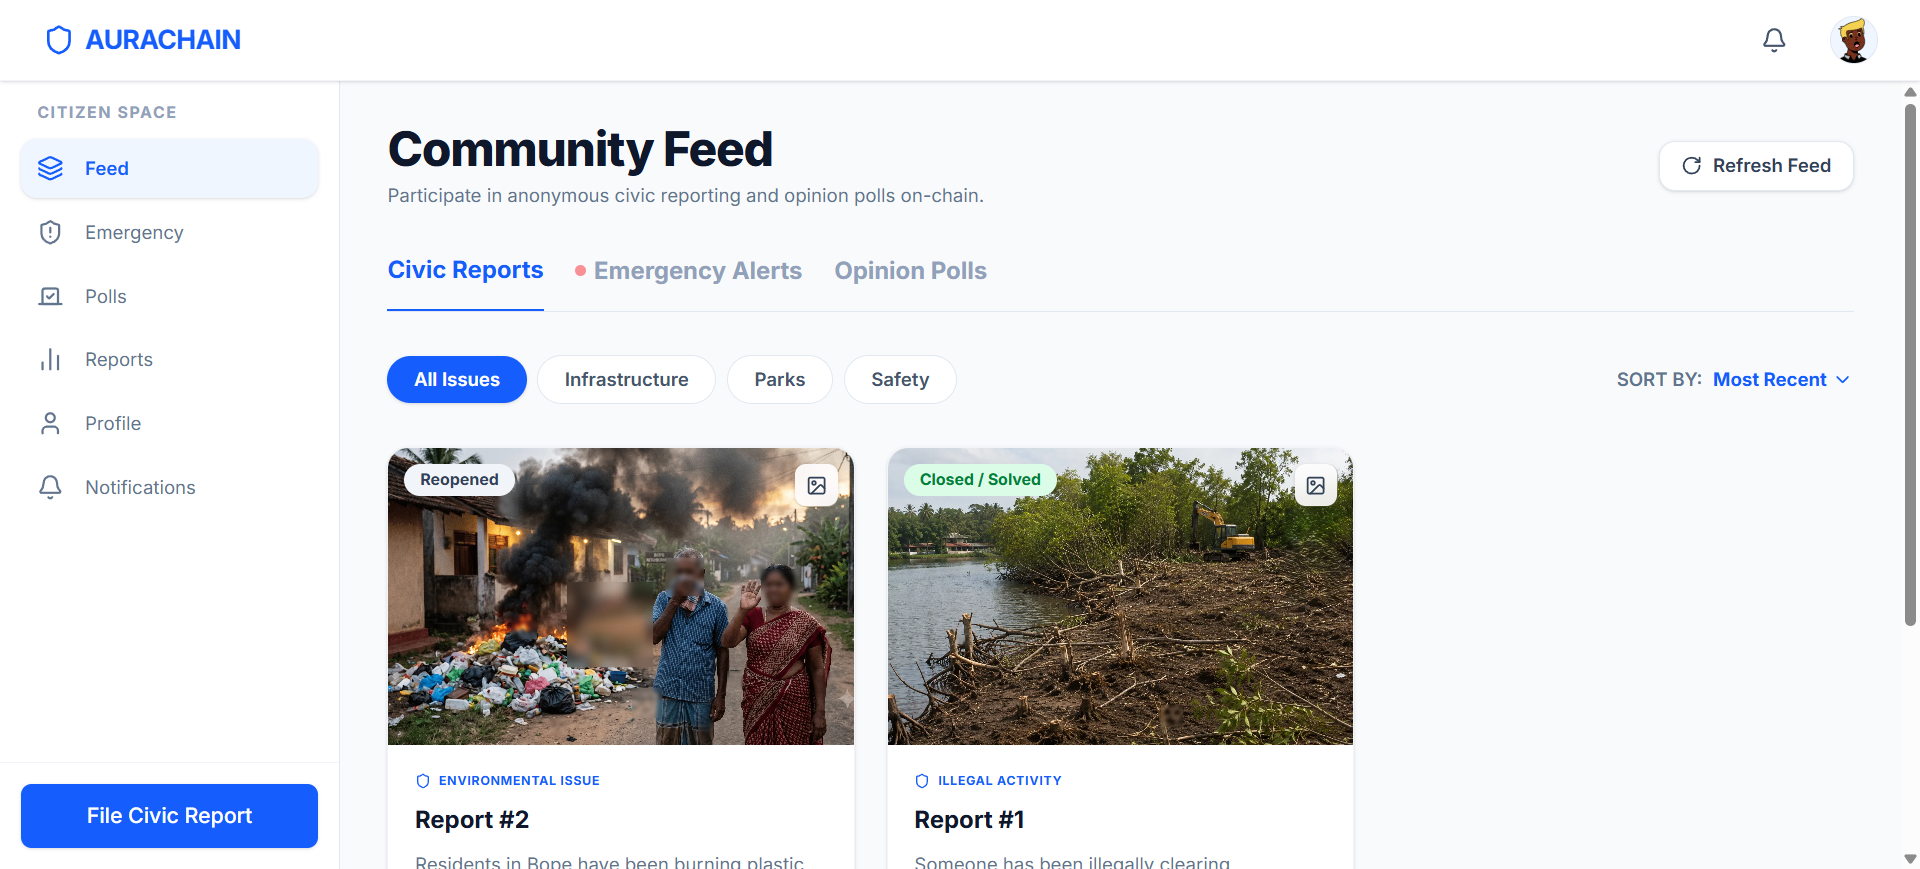
\includegraphics[width=0.85\textwidth]{Images/Appendix/me2e/feed.png}
    %\fbox{\parbox{0.85\textwidth}{\centering\vspace{3.5cm}[Screenshot M1.1-a: Citizen login]\vspace{3.5cm}}}
    \caption{Citizen feed after successful authentication}
    \label{fig:me2e-feed}
\end{figure}



% \begin{figure}[H]
%     \centering
%     % \includegraphics[width=0.85\textwidth]{Images/Appendix/m1-1-feed.png}
%     \fbox{\parbox{0.85\textwidth}{\centering\vspace{3.5cm}[Screenshot M1.1-b: Citizen feed after login]\vspace{3.5cm}}}
%     \caption{Citizen feed after successful authentication (scenario M1.1)}
%     \label{fig:m1-1-feed}
% \end{figure}

% \begin{figure}[H]
%     \centering
%     % \includegraphics[width=0.85\textwidth]{Images/Appendix/m1-2-pin.png}
%     \fbox{\parbox{0.85\textwidth}{\centering\vspace{3.5cm}[Screenshot M1.2: PIN create or unlock]\vspace{3.5cm}}}
%     \caption{Session PIN create or unlock screen (scenario M1.2)}
%     \label{fig:m1-2-pin}
% \end{figure}

% \begin{figure}[H]
%     \centering
%     % \includegraphics[width=0.85\textwidth]{Images/Appendix/m1-3-invalid.png}
%     \fbox{\parbox{0.85\textwidth}{\centering\vspace{3.5cm}[Screenshot M1.3: Invalid credentials error]\vspace{3.5cm}}}
%     \caption{Invalid citizen credentials error (scenario M1.3)}
%     \label{fig:m1-3-invalid}
% \end{figure}

% \begin{figure}[H]
%     \centering
%     % \includegraphics[width=0.85\textwidth]{Images/Appendix/m1-4-admin.png}
%     \fbox{\parbox{0.85\textwidth}{\centering\vspace{3.5cm}[Screenshot M1.4: Authority dashboard]\vspace{3.5cm}}}
%     \caption{Authority dashboard after MetaMask connection (scenario M1.4)}
%     \label{fig:m1-4-admin}
% \end{figure}

% \begin{figure}[H]
%     \centering
%     % \includegraphics[width=0.85\textwidth]{Images/Appendix/m1-5-denied.png}
%     \fbox{\parbox{0.85\textwidth}{\centering\vspace{3.5cm}[Screenshot M1.5: Access denied to /admin]\vspace{3.5cm}}}
%     \caption{Access denied when a non-authority user opens the authority portal (scenario M1.5)}
%     \label{fig:m1-5-denied}
% \end{figure}

% \begin{figure}[H]
%     \centering
%     % \includegraphics[width=0.85\textwidth]{Images/Appendix/m1-6-guard.png}
%     \fbox{\parbox{0.85\textwidth}{\centering\vspace{3.5cm}[Screenshot M1.6: Guarded citizen route]\vspace{3.5cm}}}
%     \caption{Unauthenticated access blocked on a citizen route (scenario M1.6)}
%     \label{fig:m1-6-guard}
% \end{figure}

\subsection{Standard Lifecycle Screenshots}

% \begin{figure}[H]
%     \centering
%     % \includegraphics[width=0.85\textwidth]{Images/Appendix/m2-1-form.png}
%     \fbox{\parbox{0.85\textwidth}{\centering\vspace{3.5cm}[Screenshot M2.1-a: Report submission form]\vspace{3.5cm}}}
%     \caption{Standard report submission form (scenario M2.1)}
%     \label{fig:m2-1-form}
% \end{figure}

% \begin{figure}[H]
%     \centering
%     % \includegraphics[width=0.85\textwidth]{Images/Appendix/m2-1-notifications.png}
%     \fbox{\parbox{0.85\textwidth}{\centering\vspace{3.5cm}[Screenshot M2.1-b: Pipeline notifications]\vspace{3.5cm}}}
%     \caption{SSE pipeline progress on the notifications page (scenario M2.1)}
%     \label{fig:m2-1-notifications}
% \end{figure}

% \begin{figure}[H]
%     \centering
%     % \includegraphics[width=0.85\textwidth]{Images/Appendix/m2-1-pending.png}
%     \fbox{\parbox{0.85\textwidth}{\centering\vspace{3.5cm}[Screenshot M2.1-c: PendingValidation status]\vspace{3.5cm}}}
%     \caption{Report detail in \texttt{PendingValidation} (scenario M2.1)}
%     \label{fig:m2-1-pending}
% \end{figure}

% \begin{figure}[H]
%     \centering
%     % \includegraphics[width=0.85\textwidth]{Images/Appendix/m2-2-vote.png}
%     \fbox{\parbox{0.85\textwidth}{\centering\vspace{3.5cm}[Screenshot M2.2-a: Validation upvote UI]\vspace{3.5cm}}}
%     \caption{Community validation voting UI (scenario M2.2)}
%     \label{fig:m2-2-vote}
% \end{figure}

% \begin{figure}[H]
%     \centering
%     % \includegraphics[width=0.85\textwidth]{Images/Appendix/m2-2-open.png}
%     \fbox{\parbox{0.85\textwidth}{\centering\vspace{3.5cm}[Screenshot M2.2-b: Open status]\vspace{3.5cm}}}
%     \caption{Report status after validation finalization (\texttt{Open}) (scenario M2.2)}
%     \label{fig:m2-2-open}
% \end{figure}

% \begin{figure}[H]
%     \centering
%     % \includegraphics[width=0.85\textwidth]{Images/Appendix/m2-3-inprogress.png}
%     \fbox{\parbox{0.85\textwidth}{\centering\vspace{3.5cm}[Screenshot M2.3-a: InProgress after Start Work]\vspace{3.5cm}}}
%     \caption{Authority Start Work moves the report to \texttt{InProgress} (scenario M2.3)}
%     \label{fig:m2-3-inprogress}
% \end{figure}

% \begin{figure}[H]
%     \centering
%     % \includegraphics[width=0.85\textwidth]{Images/Appendix/m2-3-pending-verif.png}
%     \fbox{\parbox{0.85\textwidth}{\centering\vspace{3.5cm}[Screenshot M2.3-b: PendingVerification]\vspace{3.5cm}}}
%     \caption{Report in \texttt{PendingVerification} after Mark as Solved (scenario M2.3)}
%     \label{fig:m2-3-pending-verif}
% \end{figure}

% \begin{figure}[H]
%     \centering
%     % \includegraphics[width=0.85\textwidth]{Images/Appendix/m2-4-closed.png}
%     \fbox{\parbox{0.85\textwidth}{\centering\vspace{3.5cm}[Screenshot M2.4: Closed status]\vspace{3.5cm}}}
%     \caption{Report closed after community verification accepts the resolution (scenario M2.4)}
%     \label{fig:m2-4-closed}
% \end{figure}

% \begin{figure}[H]
%     \centering
%     % \includegraphics[width=0.85\textwidth]{Images/Appendix/m2-5-profile.png}
%     \fbox{\parbox{0.85\textwidth}{\centering\vspace{3.5cm}[Screenshot M2.5-a: Citizen profile]\vspace{3.5cm}}}
%     \caption{Citizen profile showing pseudonym and tickets (scenario M2.5)}
%     \label{fig:m2-5-profile}
% \end{figure}

% \begin{figure}[H]
%     \centering
%     % \includegraphics[width=0.85\textwidth]{Images/Appendix/m2-5-myreports.png}
%     \fbox{\parbox{0.85\textwidth}{\centering\vspace{3.5cm}[Screenshot M2.5-b: My reports]\vspace{3.5cm}}}
%     \caption{My Reports list for the authenticated citizen (scenario M2.5)}
%     \label{fig:m2-5-myreports}
% \end{figure}

\subsection{Alternate and Negative-Path Screenshots}

% \begin{figure}[H]
%     \centering
%     % \includegraphics[width=0.85\textwidth]{Images/Appendix/m3-1-rejected.png}
%     \fbox{\parbox{0.85\textwidth}{\centering\vspace{3.5cm}[Screenshot M3.1: CommunityRejected]\vspace{3.5cm}}}
%     \caption{Report status \texttt{CommunityRejected} after validation downvotes (scenario M3.1)}
%     \label{fig:m3-1-rejected}
% \end{figure}

% \begin{figure}[H]
%     \centering
%     % \includegraphics[width=0.85\textwidth]{Images/Appendix/m3-2-review.png}
%     \fbox{\parbox{0.85\textwidth}{\centering\vspace{3.5cm}[Screenshot M3.2-a: PendingRejectionReview]\vspace{3.5cm}}}
%     \caption{Report in \texttt{PendingRejectionReview} after authority reject (scenario M3.2)}
%     \label{fig:m3-2-review}
% \end{figure}

% \begin{figure}[H]
%     \centering
%     % \includegraphics[width=0.85\textwidth]{Images/Appendix/m3-2-closed.png}
%     \fbox{\parbox{0.85\textwidth}{\centering\vspace{3.5cm}[Screenshot M3.2-b: Closed after uphold]\vspace{3.5cm}}}
%     \caption{Report closed after community upholds the authority rejection (scenario M3.2)}
%     \label{fig:m3-2-closed}
% \end{figure}

% \begin{figure}[H]
%     \centering
%     % \includegraphics[width=0.85\textwidth]{Images/Appendix/m3-3-reopened.png}
%     \fbox{\parbox{0.85\textwidth}{\centering\vspace{3.5cm}[Screenshot M3.3: Reopened after appeal]\vspace{3.5cm}}}
%     \caption{Report \texttt{Reopened} after community appeals the rejection (scenario M3.3)}
%     \label{fig:m3-3-reopened}
% \end{figure}

% \begin{figure}[H]
%     \centering
%     % \includegraphics[width=0.85\textwidth]{Images/Appendix/m3-4-verif-reopen.png}
%     \fbox{\parbox{0.85\textwidth}{\centering\vspace{3.5cm}[Screenshot M3.4: Reopened after verification reject]\vspace{3.5cm}}}
%     \caption{Report \texttt{Reopened} after verification reject majority (scenario M3.4)}
%     \label{fig:m3-4-verif-reopen}
% \end{figure}

% \begin{figure}[H]
%     \centering
%     % \includegraphics[width=0.85\textwidth]{Images/Appendix/m3-5-validation.png}
%     \fbox{\parbox{0.85\textwidth}{\centering\vspace{3.5cm}[Screenshot M3.5: Client validation error]\vspace{3.5cm}}}
%     \caption{Client-side validation preventing an invalid submission (scenario M3.5)}
%     \label{fig:m3-5-validation}
% \end{figure}

% \begin{figure}[H]
%     \centering
%     % \includegraphics[width=0.85\textwidth]{Images/Appendix/m3-6-ai-reject.png}
%     \fbox{\parbox{0.85\textwidth}{\centering\vspace{3.5cm}[Screenshot M3.6: AI rejection in notifications]\vspace{3.5cm}}}
%     \caption{AI moderation rejection shown in notifications (scenario M3.6)}
%     \label{fig:m3-6-ai-reject}
% \end{figure}

% \begin{figure}[H]
%     \centering
%     % \includegraphics[width=0.85\textwidth]{Images/Appendix/m3-7-duplicate.png}
%     \fbox{\parbox{0.85\textwidth}{\centering\vspace{3.5cm}[Screenshot M3.7: Duplicate warning modal]\vspace{3.5cm}}}
%     \caption{Duplicate geo and category warning modal (scenario M3.7)}
%     \label{fig:m3-7-duplicate}
% \end{figure}

% \begin{figure}[H]
%     \centering
%     % \includegraphics[width=0.85\textwidth]{Images/Appendix/m3-8-double-vote.png}
%     \fbox{\parbox{0.85\textwidth}{\centering\vspace{3.5cm}[Screenshot M3.8: Double-vote or ticket error]\vspace{3.5cm}}}
%     \caption{Double-vote or ticket-exhaustion error (scenario M3.8)}
%     \label{fig:m3-8-double-vote}
% \end{figure}

\subsection{Emergency Screenshots}

% \begin{figure}[H]
%     \centering
%     % \includegraphics[width=0.85\textwidth]{Images/Appendix/m4-1-consent.png}
%     \fbox{\parbox{0.85\textwidth}{\centering\vspace{3.5cm}[Screenshot M4.1-a: Emergency consent modal]\vspace{3.5cm}}}
%     \caption{Emergency consent modal before submission (scenario M4.1)}
%     \label{fig:m4-1-consent}
% \end{figure}

% \begin{figure}[H]
%     \centering
%     % \includegraphics[width=0.85\textwidth]{Images/Appendix/m4-1-open.png}
%     \fbox{\parbox{0.85\textwidth}{\centering\vspace{3.5cm}[Screenshot M4.1-b: Emergency Open status]\vspace{3.5cm}}}
%     \caption{Emergency report in \texttt{Open} without validation (scenario M4.1)}
%     \label{fig:m4-1-open}
% \end{figure}

% \begin{figure}[H]
%     \centering
%     % \includegraphics[width=0.85\textwidth]{Images/Appendix/m4-2-resolved.png}
%     \fbox{\parbox{0.85\textwidth}{\centering\vspace{3.5cm}[Screenshot M4.2: Emergency Resolved]\vspace{3.5cm}}}
%     \caption{Emergency report resolved by authority (scenario M4.2)}
%     \label{fig:m4-2-resolved}
% \end{figure}

% \begin{figure}[H]
%     \centering
%     % \includegraphics[width=0.85\textwidth]{Images/Appendix/m4-3-reclassified.png}
%     \fbox{\parbox{0.85\textwidth}{\centering\vspace{3.5cm}[Screenshot M4.3: Reclassified]\vspace{3.5cm}}}
%     \caption{False emergency reclassified by authority (scenario M4.3)}
%     \label{fig:m4-3-reclassified}
% \end{figure}

% \begin{figure}[H]
%     \centering
%     % \includegraphics[width=0.85\textwidth]{Images/Appendix/m4-4-penalty.png}
%     \fbox{\parbox{0.85\textwidth}{\centering\vspace{3.5cm}[Screenshot M4.4: Emergency penalty block]\vspace{3.5cm}}}
%     \caption{Second emergency blocked while the citizen is under penalty (scenario M4.4)}
%     \label{fig:m4-4-penalty}
% \end{figure}

% \begin{figure}[H]
%     \centering
%     % \includegraphics[width=0.85\textwidth]{Images/Appendix/m4-5-cancel-consent.png}
%     \fbox{\parbox{0.85\textwidth}{\centering\vspace{3.5cm}[Screenshot M4.5: Cancelled emergency consent]\vspace{3.5cm}}}
%     \caption{Emergency submission cancelled without consent (scenario M4.5)}
%     \label{fig:m4-5-cancel-consent}
% \end{figure}

\subsection{Polling Screenshots}

% \begin{figure}[H]
%     \centering
%     % \includegraphics[width=0.85\textwidth]{Images/Appendix/m5-1-create.png}
%     \fbox{\parbox{0.85\textwidth}{\centering\vspace{3.5cm}[Screenshot M5.1-a: Create poll form]\vspace{3.5cm}}}
%     \caption{Authority create-poll form (scenario M5.1)}
%     \label{fig:m5-1-create}
% \end{figure}

% \begin{figure}[H]
%     \centering
%     % \includegraphics[width=0.85\textwidth]{Images/Appendix/m5-1-list.png}
%     \fbox{\parbox{0.85\textwidth}{\centering\vspace{3.5cm}[Screenshot M5.1-b: Poll list]\vspace{3.5cm}}}
%     \caption{Poll visible to citizens after creation (scenario M5.1)}
%     \label{fig:m5-1-list}
% \end{figure}

% \begin{figure}[H]
%     \centering
%     % \includegraphics[width=0.85\textwidth]{Images/Appendix/m5-2-vote.png}
%     \fbox{\parbox{0.85\textwidth}{\centering\vspace{3.5cm}[Screenshot M5.2-a: Citizen poll vote]\vspace{3.5cm}}}
%     \caption{Citizen casting a poll vote (scenario M5.2)}
%     \label{fig:m5-2-vote}
% \end{figure}

% \begin{figure}[H]
%     \centering
%     % \includegraphics[width=0.85\textwidth]{Images/Appendix/m5-2-finalized.png}
%     \fbox{\parbox{0.85\textwidth}{\centering\vspace{3.5cm}[Screenshot M5.2-b: Finalized poll]\vspace{3.5cm}}}
%     \caption{Poll after authority finalization (scenario M5.2)}
%     \label{fig:m5-2-finalized}
% \end{figure}

% \begin{figure}[H]
%     \centering
%     % \includegraphics[width=0.85\textwidth]{Images/Appendix/m5-3-denied.png}
%     \fbox{\parbox{0.85\textwidth}{\centering\vspace{3.5cm}[Screenshot M5.3: Poll create access denied]\vspace{3.5cm}}}
%     \caption{Citizen denied access to poll creation (scenario M5.3)}
%     \label{fig:m5-3-denied}
% \end{figure}

\subsection{Super Admin Screenshots}

% \begin{figure}[H]
%     \centering
%     % 
\includegraphics[width=0.85\textwidth]{Images/Appendix/m6-1-propose.png}
%     \fbox{\parbox{0.85\textwidth}{\centering\vspace{3.5cm}[Screenshot M6.1-a: Super Admin proposal]\vspace{3.5cm}}}
%     \caption{Super Admin governance proposal form (scenario M6.1)}
%     \label{fig:m6-1-propose}
% \end{figure}

% \begin{figure}[H]
%     \centering
%     % 
\includegraphics[width=0.85\textwidth]{Images/Appendix/m6-1-executed.png}
%     \fbox{\parbox{0.85\textwidth}{\centering\vspace{3.5cm}[Screenshot M6.1-b: Executed proposal]\vspace{3.5cm}}}
%     \caption{Proposal executed after majority quorum (scenario M6.1)}
%     \label{fig:m6-1-executed}
% \end{figure}

% \begin{figure}[H]
%     \centering
%     % \includegraphics[width=0.85\textwidth]{Images/Appendix/m6-2-denied.png}
%     \fbox{\parbox{0.85\textwidth}{\centering\vspace{3.5cm}[Screenshot M6.2: Super Admin access denied]\vspace{3.5cm}}}
%     \caption{Non--Super Admin denied access to the Super Admin dashboard (scenario M6.2)}
%     \label{fig:m6-2-denied}
% \end{figure}
